\documentclass[10pt]{beamer}

\usetheme{metropolis}
\definecolor{WiLabRed}{RGB}{197,18,48}
\setbeamercolor{frametitle}{fg=white,bg=WiLabRed}
\setbeamercolor{progress bar}{fg=WiLabRed!90}
\setbeamercolor{title separator}{fg=WiLabRed!90}
\setbeamercolor{progress bar in section page}{fg=WiLabRed!90}
\setbeamercolor{background canvas}{bg=white}
\setbeamercolor{alerted text}{fg=WiLabRed!90}

\usepackage{appendixnumberbeamer}

\usepackage{booktabs}
\usepackage[scale=2]{ccicons}

\usepackage{pgfplots}
\usepgfplotslibrary{dateplot}

\usepackage{xspace}
\newcommand{\themename}{\textbf{\textsc{metropolis}}\xspace}

\usepackage{marvosym}
%\usepackage{subfig}
\usepackage{graphicx}\graphicspath{{images/}}
%\usepackage{subcaption}
\usepackage[framed]{mcode}
\usepackage{listings}

\usepackage{amsmath}

\title{Lecture 18: Signal Detection}
\subtitle{\textit{Software Defined Radio for Engineers} (Collins~\textit{et al.}), \textsection{8.2.1}}
\date{}
\author{\textbf{Alexander M. Wyglinski, Ph.D.}}
\institute{ \vspace*{1in}\hfill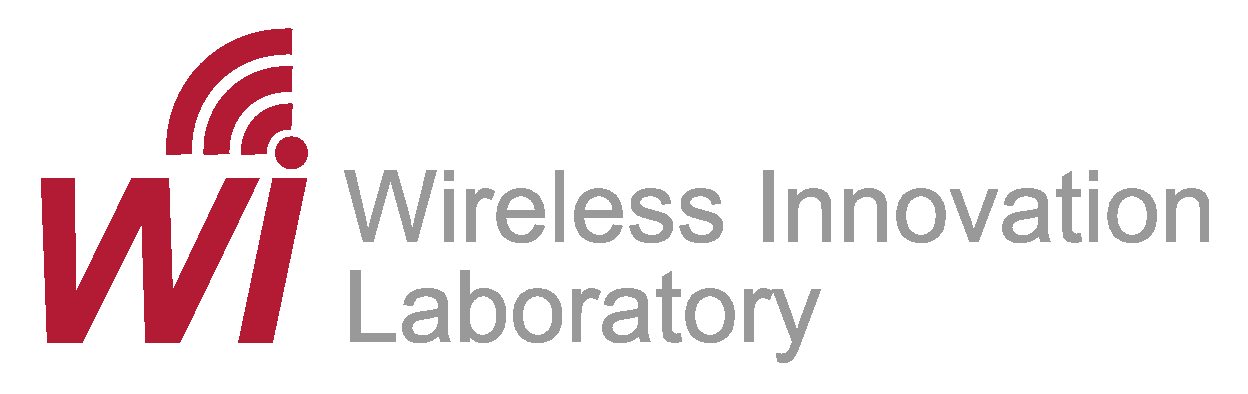
\includegraphics[height=1.125cm]{wilab_logo-A70916.eps} \qquad 
\includegraphics[height=1.125cm]{WPI_Inst_Prim_FulClr.eps}}
% \titlegraphic{\hfill\includegraphics[height=1.5cm]{logo.pdf}}

% Foot for all slides
\setbeamertemplate{frame footer}{\tiny \copyright~2018 by Alexander Wyglinski. This work is licensed under the Creative Commons Attribution-ShareAlike 4.0 International License. To view a copy of this license, visit http://creativecommons.org/licenses/by-sa/4.0/.}

\begin{document}

%\captionsetup[subfigure]{labelformat=empty}

%%%%%%%%%%%%%%%%%%%%%%%%%%%%%%%%%%%%%%%%%%%%%%%%%%%%%%%%%%

\maketitle




%%%%%%%%%%%%%%%%%%%%%%%%%%%%%%%%%%%%%%%%%%%%%%%%%%%%%%%%%%

\frame
{
  \frametitle{Hypothesis Testing}

\begin{equation}
        \begin{split}
            H_0:&~\mathrm{Null~Hypothesis}\\
            H_1:&~\mathrm{Alternate~Hypothesis}
        \end{split}
\end{equation}

\vspace*{1cm}
$\rightarrow$~What does this mean?


}

\frame
{
  \frametitle{Mathematical Context}

    \begin{itemize}
        \item \textit{Null hypothesis} represents noise with no primary signal being present
         \item \textit{Alternative hypothesis} is superposition of noise and signal of interest
          \item This can be represented as:
           \begin{equation}
        \begin{split}
            H_0:&~r[n] = n[n]\\
            H_1:&~r[n] = x[n] + n[n]
        \end{split}
        \end{equation}
        where $r[n]$ is received signal, $x[n]$ is signal of interest, and $n[n]$ is noise
    \end{itemize}

}

\frame
{
  \frametitle{Decision Rule}

    \begin{itemize}
        \item Based on observed $r[n]$, we assign two statistical scenarios for observations:
        \begin{equation}
            \delta (x)=\begin{cases}
                        1,\quad{x\in{\tau_1}}\\
                        0,\quad{x\in{\tau_1^c}}
                       \end{cases}
        \end{equation}
    \end{itemize}

}

\frame
{
  \frametitle{Decision Errors}

    \begin{itemize}
        \item Two errors can be made
        \begin{itemize}
          \item $H_0$ being falsely rejected
          \item $H_1$ being falsely rejected
        \end{itemize}
        \item Type I Error: Signal detected even when no signal present 
        \item Type II Error: Signal not detected even when signal present
        \item Commonly they are referred to as \textit{false alarm} and \textit{missed detection}
    \end{itemize}

}

\frame
{
  \frametitle{Detector Performance}

    \begin{itemize}
        \item We characterize performance of detector using probability of two errors
        \item The definition of each and the expression of performance is given as:
        \begin{itemize}
        \item \textit{Probability of False alarm}
        \begin{equation}
            P_F = P(H_1|H_0)
        \end{equation}
	\item \textit{Probability of Missed Detection}
        \begin{equation}
        P_M = P(H_0|H_1)
        \end{equation}
        \item \textit{Probability of Detection}
        \begin{equation}
        P_D = 1-P_M = P(H_1|H_1)
        \end{equation}
        \end{itemize}
    \end{itemize}

}

\frame
{
  \frametitle{Receiver Operating Characteristics}

    \begin{itemize}
        \item Ideally, we want $P_F$ to be small and $P_D$ to be large 
        \item However, they constrain each other making it impossible to be ideal
        \item Their relationship is called a \textit{receiver operating characteristic}
            \begin{itemize}
        \item This becomes a thresholding problem
	\item Need self-normalization to solve this problem
    \end{itemize}
    \end{itemize}

}

\frame
{
  \frametitle{Self-Normalization}
    \begin{itemize}
        \item We force signal to range closely between [0,1]  
\item Achieved by scaling cross-correlation metric via mean energy of input signal
	\item Mathematically, this is expressed as:
        \begin{equation}
          u_{ma}[n] = \sum\limits_{i=1}^{N} u[n-i]
        \end{equation}
        where $N$ is the length of the preamble
        \item Implementation of moving average filter
    \end{itemize}
}


\frame
{
  \frametitle{Modified Expressions }
    \begin{itemize}
	\item Frame synchronization system may also be used for packet detection
	\item Detector is given by:
	\begin{equation}
        \begin{split}
            H_0:&~y[n]/u_{ma}[n]<T\hspace{1ex}\rightarrow\mathrm{no~signals}\\
           H_1:&~y[n]/u_{ma}[n]\geq{T}\hspace{1ex}\rightarrow\mathrm{signals~exist}
        \end{split}
        \end{equation}
        where $T$ is threshold Value
    \end{itemize}
}







\end{document}
